% Chapter 2
% Roberto Masocco <robmasocco@gmail.com>
% August 28, 2021

\chapter[Nuovi problemi e nuove soluzioni]{Nuovi problemi e nuove soluzioni}
\label{chap:Chapter2}
\doublespacing
\fontsize{14}{14}\selectfont

\newsection{Premessa}
\indent Lo sviluppo di un sistema robotico autonomo è un processo che attraversa varie fasi. Ciascuna di esse è solitamente caratterizzata dalla definizione e soluzione di problematiche inerenti diversi aspetti dell'apparato, che possono andare dalle operazioni che questo sarà chiamato a svolgere, alla sua costruzione e programmazione, fino al modo in cui i dati che esso raccoglie e che condizionano il suo funzionamento debbano essere presentati agli eventuali operatori. Volendo generalizzare dallo specifico caso applicativo, la maggior parte delle problematiche si possono ripartire tra poche tipologie di alto livello. Nonostante possa risultare controintuitivo dalla suddivisione che ci si appresta a delineare, queste non sempre si rivelano affrontabili in sequenza, né tanto meno completamente indipendenti. È anche per risolvere situazioni simili che negli ultimi tempi sono state ideate svariate tecniche di project management, volte anche a minimizzare il rischio che un errore commesso in una fase precedente possa pregiudicare quelle future, compromettendo il lavoro svolto ed allungando i tempi di sviluppo. In virtù di quanto osservato nel capitolo precedente, è chiaro che con l'aumentare della complessità dei sistemi automatici odierni e dei compiti che essi devono svolgere, queste tematiche siano quanto mai attuali. In particolare, nuovi strumenti messi a disposizione di sviluppatori e progettisti dovranno riflettere queste specificità, semplificare la gestione di situazioni tipiche dove possibile, ed evidenziare eventuali criticità per aiutare nella soluzione dei problemi. Nonostante la generalizzazione che si sta facendo possa sembrare eccessiva, nella realtà pratica si riscontra facilmente che a dispetto della varietà di casi di specie e applicazioni, le complicazioni da affrontare sono quasi sempre se non le stesse, molto simili, e lo stesso si può rilevare circa le strategie da adottare.\\
L'obiettivo di questo capitolo è presentare brevemente le problematiche che solitamente si devono affrontare quando si progetta un sistema robotico, evidenziandone le peculiarità seppur senza concentrarsi su un particolare ambito applicativo, e passare poi ad esaminare alcune recenti soluzioni hardware e software che consentono di ottimizzare il lavoro di progettazione, sviluppo e testing in loro funzione. La discussione parte ora da un livello abbastanza alto di astrazione ma diventerà via via sempre più specifica, costituendo di fatto la linea guida seguita durante il progetto che costituisce il caso di studio di questo lavoro e dunque un filo che lega tutti i capitoli successivi.

\newsection{Fasi e criticità progettuali}
\newsubsection{I task}
\indent Le prime decisioni da prendere all'inizio del progetto di un sistema automatico o robotico riguardano naturalmente le specifiche delle operazioni che questo dovrà svolgere. Esse vanno completamente delineate fin da subito nei minimi particolari, in quanto è da loro che dipenderanno tutte le scelte successive, da quelle inerenti la costruzione e la scelta dell'hardware fino alla sua programmazione. Durante questa decomposizione dei requisiti operativi in \emph{task}, intesi come singole unità di lavoro da eseguire, compariranno diversi tipi di questi ultimi. Senza scendere, per ora, nei particolari di uno specifico caso, tipologie comuni sono:
\begin{itemize}
    \item task \textbf{continuativi}, ossia iniziati all'accensione del sistema e mai interrotti fino al suo spegnimento o malfunzionamento;
    \item task \textbf{periodici}, da eseguire a intervalli regolari;
    \item task \textbf{asincroni}, svolti solo quando un particolare evento si verifica.
\end{itemize}
È facile rendersi conto di come gran parte delle funzionalità presenti nei sistemi robotici odierni possa essere decomposta in task appartenenti a ciascuna di queste categorie. Ne fanno evidentemente parte operazioni che vanno dal controllo degli attuatori, alla raccolta di dati e misure necessari agli algoritmi di controllo, fino alla comunicazione con operatori ed utenti. Le specificità di questi task avranno risvolti sia sull'hardware che dovrà realizzarli che sul software che li codificherà, i quali dovranno essere organizzati opportunamente in loro funzione, anche in modo da facilitarne lo sviluppo e la manutenzione.

\newsubsection{L'hardware}
\indent Le decisioni da prendere successivamente riguardano l'hardware da utilizzare per realizzare i primi prototipi dell'apparato. Probabilmente non si tratterà di quello che comporrà il prodotto finito, per via di eventuali errori di valutazione, imprevisti o altre problematiche sorte successivamente. Ciò nonostante esso deve essere selezionato con cura in base ai requisiti operativi, strutturali e costruttivi definiti fin qui. Le decisioni prese durante il passo precedente rivestono in questa fase un'importanza cruciale: stabilendo infatti quale sia la complessità computazionale delle operazioni che il sistema dovrà svolgere, sarà richiesto un hardware di alto livello più o meno potente, equipaggiato eventualmente con coprocessori discreti\footnote{Con il termine \emph{discreto} si intende hardware aggiuntivo montato su di un calcolatore, non in grado di operare da solo ma fatto per essere pilotato da quest'ultimo, offrendogli supporto specifico per particolari operazioni; classici esempi sono i coprocessori matematici, le GPU e le schede audio.} necessari per trattare particolari tipi di dati, o suddiviso in più sottosistemi interconnessi. Al giorno d'oggi, ricordando la discussione fatta nel capitolo precedente circa la disponibilità di un'ampia gamma di soluzioni off-the-shelf, è d'obbligo un'indagine di ciò che offre il mercato per capire se sia possibile sfruttare componenti o SoC forniti già testati e pronti per essere utilizzati, piuttosto che ricorrere ad una soluzione proprietaria che porta generalmente con sé considerevoli costi di sviluppo, testing e validazione. Per i motivi sopracitati è molto difficile, se non impossibile, delineare fin da questo punto una struttura complessiva e definitiva dell'hardware: ciò che importa è capire di cosa c'è bisogno e se esistono sul mercato offerte compatibili con i propri requisiti, cercando di prevedere anche successive richieste aggiuntive. Seguendo questa linea, eventuali variazioni potranno essere gestite similmente con poco sforzo.\newpage
Il resto delle scelte riguardano l'hardware di più basso livello, formato in generale da:
\begin{itemize}
    \item microcontrollori veloci;
    \item attuatori;
    \item sensori;
    \item interfacce e dispositivi di comunicazione;
    \item hardware per il controllo e la supervisione;
    \item sistemi di immagazzinamento di dati.
\end{itemize}
Niente di più si può dire su di esse prescindendo dal caso di specie, tuttavia nel seguito di questo lavoro saranno descritte situazioni simili relative all'esempio che si discuterà. Per ora ci si può limitare a sottolineare che le osservazioni fatte precedentemente valgono anche per questi componenti.

\newsubsection{Il software}
\indent Eccezion fatta per quei componenti che svolgono funzioni cruciali e molto specifiche, come circuiti elettrici/elettronici, la quasi totalità delle operazioni svolte da un sistema robotico è oggi codificata in un calcolatore ad esso interno, che traduce tali istruzioni in comandi per gli altri componenti, sottosistemi, sensori o attuatori. Non è questa la sede per la discussione di procedure standard di progettazione e realizzazione del software, ma basta soffermarsi a riflettere su un punto: anche il software che governa un robot, data la complessità di quest'ultimo, avrà un'organizzazione stratificata e fortemente gerarchica. In essa, i livelli inferiori saranno occupati da quei moduli che dovranno interagire con, se non muovere, i sottosistemi più piccoli e veloci (e.g. il \emph{firmware}), e che andranno sviluppati ponendo particolare attenzione alle caratteristiche di essi ed alle loro finalità. Man mano che si sale nella scala gerarchica ci si muove verso moduli a più ampio spettro, che codificano operazioni di supervisione, pianificazione e comunicazione con gli utenti, e per questo più vicini alla nozione di software applicativo o di sistema, con cui magari si è più abituati ad avere a che fare essendo quello "maggiormente visibile" ad un utente finale. Supponendo di dover operare in questo contesto, si deve poter contare su degli strumenti che semplifichino il più possibile il design e lo sviluppo a tutti i livelli senza distinzione, aiutando nella gestione di problematiche inerenti l'organizzazione dei moduli, la comunicazione, il processamento e la memorizzazione di diversi tipi di dati.\\
Rientra in questo contesto anche una decisione circa i linguaggi di programmazione da adottare. Com'è noto, ciascuno possiede le sue caratteristiche peculiari, che ne evidenziano rispetto alle alternative punti di forza ma anche debolezze. Pochi sono i linguaggi di programmazione adatti per molteplici scopi, intendendo in questo senso il grado di facilità con cui consentono di codificare diversi tipi di task, e nessuno è da considerarsi universale. Nel seguito di questo lavoro verranno presentate, a titolo di esempio, due diverse alternative, mettendone in risalto le specificità e motivando un uso preponderante di una delle due con dei requisiti progettuali del caso di studio.\newpage

\newsubsection{I dati e le misure}
\indent Un robot, per portare a termine i propri task con successo, necessita più o meno costantemente di informazioni circa quello che gli sta accadendo intorno. Esse possono essere ricevute entro pacchetti dati, gestiti da opportune interfacce di comunicazione, oppure acquisite direttamente mediante degli organi di misurazione, comunemente detti \emph{sensori}. Per entrambe queste soluzioni, problematiche classiche che si incontrano da subito sono l'integrazione dei relativi dispositivi nel resto dell'apparato e il processamento dei dati che queste restituiscono. Esse sono peraltro cruciali, in quanto il funzionamento dell'intero apparato è quasi sempre condizionato alla possibilità di disporre di informazioni circa l'ambiente circostante e lo stato del robot stesso\footnote{Si pensi agli algoritmi di controllo in \emph{feedback}, basati sulla possibilità di acquisire misure delle azioni di controllo impartite ad un sistema e di grandezze che ne esplicitano gli effetti.}. E' dunque lecito aspettarsi che un robot sia dotato di una gran quantità di interfacce di comunicazione e sensori, questi ultimi composti da hardware specifico atto a misurare particolari grandezze fisiche d'interesse. Le due problematiche introdotte poco fa riguardano pertanto l'integrazione di tale hardware con il resto del sistema e la scrittura di moduli software capaci di gestirlo, e ricevere e processare i dati che produce. Sia le piattaforme hardware che gli strumenti software dovrebbero essere sviluppati o scelti, per quanto possibile, tenendo conto di queste eventualità in modo da minimizzarne l'impatto e facilitare il lavoro.\newpage

\newsubsection{Debugging, testing e deployment}
\indent Non appena i primi prototipi vengono finalizzati occorre iniziare a testarli per verificarne il funzionamento e confermare la validità delle decisioni progettuali prese fino a quel punto. Tenendo presente che non si può definire una procedura di testing generica e universale per qualunque tipo di sistema robotico, ci si può aspettare che non appena si è constatato il corretto funzionamento dell'hardware, si debba passare alla validazione del software. Il debugging del software in esecuzione su un robot è in generale più difficile rispetto a quello di un comune software applicativo, e ciò a causa di diverse specificità:
\begin{itemize}
    \item è più difficile tracciare l'esecuzione di programmi su un dispositivo autonomo, potenzialmente in movimento: non è detto che si abbia accesso diretto al sistema e tipicamente gli strumenti a disposizione sono limitati o non molto sofisticati;
    \item in caso di problemi, oltre al software va ricontrollato anche l'hardware in uso, in quanto il problema potrebbe anche essere causato da quest'ultimo o da un suo uso non corretto;
    \item eseguire test non è semplice quanto lanciare un programma e controllarne gli esiti: va assicurata anche la sicurezza dell'apparato e dei suoi operatori durante l'intera procedura, motivo per cui già la sola organizzazione di un test può risultare impegnativa.
\end{itemize}
Date la difficoltà e l'importanza di questa fase, è ragionevole voler impiegare strumenti e metodologie che possibilmente facilitino le cose anche a questo livello, che magari siano già state adeguatamente validate e certificate.\\
Infine si può passare al \emph{deployment}, ossia la costruzione di un apparato che si possa considerare un prodotto finito da mettere in uso. È questo il momento in cui si manifestano le conseguenze di alcune scelte progettuali che in questa sede si è scelto di non trattare, relative ad esempio alla produzione e realizzazione delle varie parti. Ciò non toglie come una ragionevole oculatezza nelle fasi precedenti possa risultare conveniente anche qui.\hfill

\vspace{\baselineskip}

\indent Alla luce della discussione appena conclusa, si rileva come le problematiche da affrontare nella realizzazione di un sistema robotico siano molteplici e variegate, come pure le scelte che si è chiamati a fare in diversi punti dello sviluppo. Le ripercussioni che queste possono avere sono pure diversificate, e rischiano di manifestarsi anche in stadi più avanzati. In tempi recenti le difficoltà delineate si sono poi acuite, proprio a causa della maggiore complessità ed autonomia demandate a tali apparati. Ciò nonostante, lo sviluppo tecnologico è proseguito, rendendo anche piccoli SoC dotati di CPU multicore performanti, RAM capiente e GPU, e capaci di integrarsi facilmente con microcontrollori numerici più veloci e sottosistemi real-time più piccoli, eseguendo task abbastanza veloci oppure più lenti, ad esempio di supervisione, coordinamento o comunicazione. Quello che resta sono le difficoltà relative alla programmazione e lo sviluppo del software dedicato.\newpage
Il resto di questo capitolo è dedicato alla discussione di nuove soluzioni, recentemente divenute interessanti in ambiti quali IoT, mobile devices e telecomunicazioni, ma che stanno trovando anche nella robotica enormi risvolti applicativi. È anche grazie ad esse che il drone autonomo descritto successivamente, esempio pratico di questo studio, è stato realizzato con relativa semplicità.

\newsection{Middleware}
\indent Nel 1968 a Garmisch, in Germania, si tenne una conferenza sponsorizzata dal Comitato Scientifico della NATO sul tema dello sviluppo del software. Nonostante non se ne parli molto, si trattò di un evento storico molto importante in questo ambito: venne fatto il punto sulle pratiche e metodologie di design seguite dalle maggiori industrie attive nel campo dell'informatica, allora in forte crescita e competizione, nel tentativo di individuare strategie standard per affrontare problemi comuni.\\
Si ricorda infatti che all'epoca, e per altri quindici anni almeno, non sarebbe esistito quasi nessuno standard da seguire nella produzione e programmazione dei calcolatori: ogni azienda proponeva il suo prodotto sviluppato da zero, nell'hardware e nel software. Solo quando le informazioni hanno iniziato ad essere scambiate tra diversi calcolatori, prima su supporti di memorizzazione e poi attraverso Internet contemporaneamente ad una domanda sempre crescente di nuovi tipi di dispositivi, è iniziata un'opera di standardizzazione e collaborazione tra i diversi produttori.\newpage
Si può trovare in \cite{middleware} una trascrizione abbastanza completa della conferenza. In essa si parla per la prima volta ufficialmente di alcuni concetti oggi ben noti, come \emph{component design} o \emph{unit test}, ma ciò che interessa ai fini di questo lavoro è la rappresentazione della struttura gerarchica del software presentata da d’Agapeyeff, valida ancora oggi a meno di dovute estensioni, con lo schema a piramide invertita riportato in Figura \ref{fig:sw_pyramid}.

\begin{figure}[h]
    \centering
    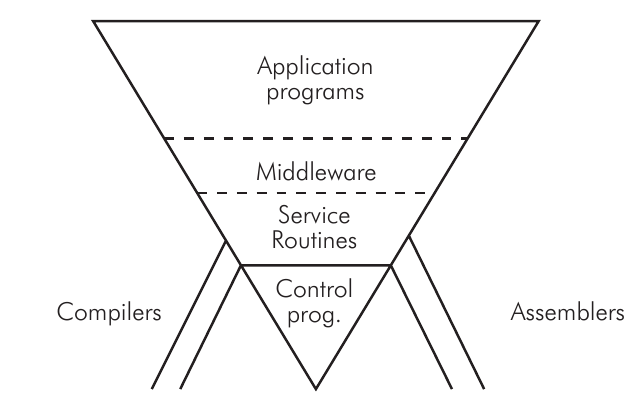
\includegraphics[width=0.9\textwidth]{figs/chapter2/software_pyramid.png}
    \caption{Organizzazione del software in esecuzione su un calcolatore generico.}
    \label{fig:sw_pyramid}
\end{figure}

L'idea è che un sistema complesso, così come una piramide invertita, non può restare operativo senza un adeguato supporto offerto da strumenti secondari, magari totalmente invisibili all'utente finale, ma che sono d'importanza vitale per il corretto funzionamento del tutto: \emph{compilatori} e \emph{assemblatori}, ossia programmi che traducono codice scritto in un qualche linguaggio prima nell'assembly dell'architettura target e poi in linguaggio macchina binario, tipicamente generando alla fine della pipeline di processamento un file eseguibile. Questi devono essere affidabili ed efficienti, poiché da essi dipende l'implementazione di tutto il resto.\\
Successivamente troviamo gli strati dei \emph{Control programs} e \emph{Service Routines}: si tratta di quelli che al giorno d'oggi siamo abituati a chiamare \emph{Sistema Operativo} e \emph{drivers}: questi vengono sviluppati solitamente a diretto contatto con la macchina, tenendone presenti le specificità, e dipendono fortemente dagli strumenti di compilazione impiegati. Il loro ruolo è quello di fornire un'astrazione dell'hardware che ne renda semplice l'utilizzo sia da parte dell'utente finale, che usa le applicazioni, sia da parte degli stessi programmatori di applicazioni. Ed il software applicativo è proprio quello che ritroviamo nell'ultimo livello: programmi che usano l'hardware più o meno direttamente per offrire agli utenti svariati servizi.\\
C'è però uno strato, intermedio, che solitamente non viene considerato poiché in passato non sempre presente o difficile da caratterizzare: il \emph{middleware}. Posizionato a metà tra il software di sistema e quello applicativo, il middleware trova la sua prima definizione e caratterizzazione proprio in occasione della suddetta conferenza. Inizialmente pensato solo come uno strato connettivo tra software corrente e \emph{legacy}, è un software che fornisce servizi e funzionalità comuni alle applicazioni al di fuori di quanto offerto dal sistema operativo. Dal punto di vista di quest’ultimo, si presenta come un normale software applicativo, composto ad esempio da librerie condivise o dinamiche. La gestione dei dati, i servizi applicativi, la messaggistica, l'autenticazione e la gestione delle API\footnote{Con \emph{Application Programming Interface} si intende un insieme di funzioni e procedure proprie di un sistema, un software o un linguaggio di programmazione, atte all'espletamento di un determinato compito. Sono generalmente implementate come librerie rese disponibili al programmatore.} sono tutti compiti comunemente assolti dal middleware, il quale dunque aiuta gli sviluppatori a creare applicazioni in modo più efficiente, agendo come tessuto connettivo tra queste ultime, i dati e gli utenti.\vfill\newpage
In ambienti distribuiti o in presenza di container\footnote{Un \emph{container} è un pacchetto di software autosufficiente, comprendente sia il proprio codice sorgente che tutte le dipendenze, dunque pronto per essere direttamente eseguito su qualunque sistema o macchina. Sono spesso usati in ambienti virtualizzati, assegnandogli in parallelo porzioni delle risorse della macchina host e isolandogli tra loro, garantendo prestazioni uniformi e predicibili e il rispetto di standard di sicurezza.}, il middleware può rendere facile e conveniente sviluppare ed eseguire applicazioni su larga scala. Un servizio generalmente offerto da un middleware è un modo per scambiare dati tra applicazioni, anche tramite dispositivi diversi, secondo un formato comune denominato \emph{interfaccia} definito al bisogno.\\
In generale, i servizi offerti sono specificati solo nei termini della loro dinamica ma possono essere portati su diverse architetture e dispositivi, funzionandovi allo stesso modo pur mantenendo la loro implementazione nascosta all’utente finale: ad esempio, quando un middleware si occupa di realizzare la comunicazione tra applicazioni, in uno stack di rete si porrebbe tra il livello di trasporto e quello di applicazione.\\
Oggi, il middleware si può dividere in due tipologie: quello che opera in \emph{tempo umano}, e dunque è pensato per essere usato direttamente da utenti umani (e.g. servizi web), e quello che opera in \emph{tempo macchina}, ed è dunque composto principalmente da API che i programmatori di applicazioni possono usare per svolgere i loro compiti con più facilità e beneficiando di una maggiore portabilità verso un'ampia varietà di dispositivi.\\
Alla luce di tutto ciò, ricordando le difficoltà che comunemente si incontrano durante il design del software di un sistema robotico, ci si può rendere conto di come l'adozione di un middleware nei sottosistemi di più alto livello possa rendere le cose più semplici: molti dei moduli che andrebbero realizzati ex novo sarebbero invece implementati dal middleware stesso e offerti sotto forma di servizi da includere nei programmi da sviluppare.\vfill\newpage

\newsection{Data Distribution Service}
\indent Nel 1989, undici compagnie tra cui Hewlett-Packard, IBM, Sun Microsystems, Apple Computer e American Airlines fondarono l’\emph{Object Management Group}, un consorzio tuttora attivo nel campo dell’informatica con il fine di definire standard per il software a scopo industriale, favorendo l’integrazione di soluzioni di vendors diversi in unici ecosistemi, relativi a differenti tipi di applicazioni e tecnologie. L’obiettivo dell'OMG è stabilire, per ogni nuova tipologia di software in esame, un modello comune da seguire nella sua implementazione, che renda possibile e favorisca il suo sviluppo ed utilizzo su potenzialmente qualunque genere di piattaforma che sia per essa rilevante.\\
Il Gruppo fornisce all’industria solo specifiche e non implementazioni, anche se un team che ne sottomette una nuova, prima che questa sia accettata, deve fornirne una possibile implementazione: ciò è, intuitivamente, per evitare di definire standard inutili o irrealizzabili. Tra le compagnie membri dell’OMG è favorito lo sviluppo di soluzioni che possano interoperare da subito e senza alcuna limitazione.\\
Uno standard definito dall’OMG è quello denominato \emph{DDS - Data Distribution Service} \cite{dds}. Esso definisce un particolare tipo di middleware, incaricato di gestire comunicazioni dirette tra sistemi real-time specificando come i dati debbano essere serializzati, deserializzati, trasmessi e instradati, e come debbano essere fatte le API che consentono ai programmatori di invocare queste operazioni. Ma c’è molto di più: l’obiettivo di un DDS è consentire a tecnologie, piattaforme e dispositivi di differenti vendors, operanti in ambiti e luoghi diversi, di comunicare da subito scambiandosi dati di cui sia noto a priori solo il formato e poco altro, consentendo di gestire criticità, prestazioni e scalabilità dei vari apparati e della rete che li collega. Di fatto, un DDS semplifica notevolmente ad un programmatore quello che sarebbe un complesso lavoro di configurazione di rete ed organizzazione delle trasmissioni, che come si è visto è una delle problematiche classiche incontrate durante la realizzazione di un sistema robotico.\\
Il modello del middleware è di tipo \emph{publish-subscribe}: le entità coinvolte nella comunicazione, denominate \emph{nodi}, dichiarano alle altre la propria volontà di trasmettere o ricevere pacchetti di informazioni, codificati secondo opportune interfacce. La ragione della denominazione sta nell'organizzazione delle diverse trasmissioni, dal punto di vista del programmatore, in \emph{topic}, ossia astrazioni che rappresentano canali di comunicazione definiti da:
\begin{itemize}
    \item un \textbf{nome} che identifichi il topic, non necessariamente in modo univoco, generalmente codificato come una stringa di testo in modo che per i programmatori sia facile ricordarlo e utilizzarlo;
    \item un'\textbf{interfaccia}, descritta secondo un qualche linguaggio (e.g. IDL\footnote{Con \emph{Interface Description Language} si intende un linguaggio con cui si possano descrivere elementi operativi che siano intelligibili da linguaggi diversi. Ne esistono vari, e in questo contesto un DDS ne fa un uso volto a rendere semplice al programmatore la specifica del formato di un pacchetto dati, nonostante nella specifica dell'OMG non sia indicato un IDL in particolare.}), che specifichi quale sia il contenuto di un singolo pacchetto di dati e come sia codificato;
    \item una policy di \textbf{Quality of Service}, specificata dal programmatore per impartire al middleware precise indicazioni su come debbano essere gestite le comunicazioni.
\end{itemize}
\vfill\newpage
Su uno stesso topic, un nodo può essere sia publisher che subscriber, e non sono vietate a priori istanze multiple di stessi topic. Riguardo il QoS, dal punto di vista dell'organizzazione delle trasmissioni sulla Rete questo riveste un ruolo importante, essendo uno strumento a disposizione del programmatore per invocare uno specifico comportamento del DDS.\\
Una policy QoS di un DDS è generalmente composta da:
\begin{itemize}
    \item \textbf{history}, impostazione che indica se vadano bufferizzati tutti i pacchetti trasmessi su un determinato topic oppure un loro numero massimo prefissato;
    \item \textbf{depth}, profondità della coda finita eventualmente impostata al punto precedente;
    \item \textbf{reliability}, che sta ad indicare se le comunicazioni vadano gestite dal middleware in modo da assicurare o meno la ricezione da parte di tutti i subscribers di un topic dei pacchetti trasmessi dai publishers;
    \item \textbf{durability}, che consente di conservare i pacchetti trasmessi da un publisher in modo da recapitarli anche ai subscribers che dovessero connettersi successivamente;
    \item \textbf{deadline}, \textbf{lifespan}, \textbf{liveliness} e \textbf{lease duration}, tempi massimi caratteristici che consentono di capire quando un pacchetto è diventato vecchio o un nodo può considerarsi non più attivo.
\end{itemize}
Chiaramente esistono delle impostazioni di default, che si cerca di mantenere il più possibile uguali tra diverse implementazioni in modo da garantire la massima compatibilità.\newpage
È evidente già a questo livello la notevole semplificazione introdotta da un middleware DDS: con una configurazione relativamente semplice e rapida si possono risolvere immediatamente problemi quali la scelta di un protocollo di trasporto (e.g. TCP o UDP) e la costruzione di moduli software che lo usino per trasmettere informazioni codificate secondo specifiche regole.\\
Il DDS si occupa di tutti i compiti necessari ad organizzare le comunicazioni: dai più basilari quali la trasmissione dei messaggi a quelli organizzativi come l’advertising dei publisher e la discovery dei nodi nella rete, al controllo di flusso e delle ritrasmissioni, gestisce la ridondanza dei publisher e altre situazioni patologiche, il tutto in modo trasparente al programmatore. Un DDS di fatto rende molto semplice costruire applicazioni distribuite, o reti di esse, in quanto nasconde e semplifica allo sviluppatore moltissimi compiti di gestione, consentendogli di prescindere totalmente da fattori che invece potrebbero risultare complessi da gestire (si pensi ai problemi che può creare la sola dislocazione geografica dei nodi).\\
I DDS oggi commercialmente disponibili offrono librerie di API in diversi linguaggi quali  Ada, C, C++, C\#, Java, Python, Scala, Lua, Pharo e Ruby, ed essendo costruiti tutti sullo stesso standard sono completamente compatibili ed interoperabili. Talvolta vengono organizzate dimostrazioni che coinvolgono diversi vendors volte a presentare e dimostrare:
\begin{itemize}
    \item funzioni di connettività di base su strato di rete con protocollo IP;
    \item discovery di publishers e subscribers;
    \item compatibilità delle comunicazioni soggette a requisiti di QoS uguali o simili;
    \item gestione dei ritardi di trasmissione;
    \item gestione di situazioni patologiche quali multiple istanze di stessi topic;
\end{itemize}
Esistono poi specifiche riguardanti tipologie di DDS di più basso livello, pensati per essere inclusi in sistemi a risorse limitate, e.g. \emph{embedded}, restando comunque compatibili con le più complete implementazioni di alto livello.\\
Le modalità di comunicazione, serializzazione e deserializzazione dei dati, sono definite nello standard OMG denominato \emph{Wire Protocol}, di cui una recentissima versione è disponibile in \cite{wire}. Nonostante l'ampiezza del contenuto, ai fini di questa trattazione è necessario evidenziarne due parti salienti.

\newsubsection{Discovery Module}
\indent Questo modulo del DDS comprende dei protocolli che consentono a diverse istanze di DDS in esecuzione su sistemi collegati in Rete di trovarsi ed organizzare le eventuali comunicazioni da quel momento in poi. Essi sono generalmente due:
\begin{itemize}
    \item \textbf{Participant Discovery Protocol (PDP)}, che consente alle istanze dei DDS, ciascuna relativa ad una qualche applicazione in esecuzione su una determinata macchina e per questo denominate \emph{participants}, di annunciare alle altre la propria esistenza ed allo stesso tempo ottenere informazioni circa eventuali altre raggiungibili;
    \newpage
    \item \textbf{Endpoint Discovery Protocol (EDP)}, chiamato in causa subito dopo il precedente e relativo alla trasmissione di informazioni che riguardano gli \emph{endpoints} che i vari participants possiedono, intesi come publishers o subscribers che risultano compatibili in quanto relativi ad uno stesso topic, una stessa interfaccia e governati da policy QoS compatibili.
\end{itemize}
Le implementazioni possono scegliere di includere, oltre ai protocolli PDP ed EDP definiti dallo standard\footnote{Essi sono noti come \textbf{SPDP} ed \textbf{SEDP} rispettivamente, dove la "S" sta per "Simple".}, delle versioni proprietarie. Se due istanze che iniziano una comunicazione hanno in comune almeno un PDP e un EDP, possono scambiarsi informazioni e completare la discovery.\\
Si tratta di protocolli che in uno stack di rete si troverebbero al livello di IP, di tipo \emph{unicast} oppure \emph{multicast} a seconda che i participants coinvolti siano tutti noti a priori o meno: nel primo caso è necessaria una configurazione di rete preliminare del DDS in modo che gli indirizzi ed i range di porte di tutte le macchine coinvolte siano preimpostati, mentre nel secondo i protocolli faranno tutto automaticamente non appena le istanze dei DDS vengono avviate. La potenzialmente vastissima scala operativa di queste soluzioni ha reso i DDS appetibili per ambiti mission-critical quali quello militare e logistico, nonostante non sia per ora consigliabile appoggiarsi interamente alla rete Internet per questo tipo di comunicazioni in quanto, a meno di configurazioni predefinite, è necessario che ogni apparato di Rete presente nel percorso tra due participants supporti il multicast e non ostacoli le trasmissioni.\vfill\newpage

\newsubsection{Platform Specific Model}
\indent Questo modello stabilisce come dati di formati e codifiche diversi debbano essere serializzati, trasmessi e deserializzati, in modo univoco per tutte le possibili implementazioni e piattaforme, tra i diversi topic.\\
Tutti i pacchetti dati sono trasportati su UDP. Indipendentemente dal fatto che l’associazione degli endpoints sia stata eseguita in multicast o unicast, il protocollo del Discovery Module avrà aperto per essi \emph{socket} UDP con numeri di porta ben precisi, dipendenti da:
\begin{itemize}
    \item \textbf{Domain ID}, costante numerica che seleziona nell'implementazione un range di porte UDP e dunque consente alle applicazioni che usano il DDS di comunicare solo specificando stessi domini; più domini possono coesistere anche entro una stessa macchina;
    \item base del range di porte UDP utilizzabili nel sistema;
    \item \textbf{Participant ID}, identificativo univoco di un'istanza entro una stessa macchina;
    \item eventuali configurazioni manuali.
\end{itemize}
Ci si potrebbe a questo punto chiedere perché usare UDP per il trasporto dei dati. Le ragioni di questa scelta sono le stesse di altri contesti simili: UDP è un protocollo basico, best-effort e privo di qualunque funzionalità di gestione della comunicazione che non sia il semplice trasporto tra endpoints, per questo leggero e dunque supportato da un'amplissima varietà di dispositivi e piattaforme; tutto ciò conferisce alle sue implementazioni una predicibilità totale, fatta ovviamente eccezione per quello che accade nella Rete, e una naturale scalabilità. Per questo è la scelta migliore sia per i sistemi real-time, sia per lo sviluppo di questo genere di software.\newpage

\newsection{Caso di studio: ROS 2}
\indent Si è discussa finora una classe di moduli software i cui obiettivi coincidono con quelli che emergono durante la progettazione di un sistema robotico, e si è passati a descriverne una tipologia specifica atta ad offrire particolari servizi di comunicazione real-time. Con tutti questi elementi a disposizione è ora possibile introdurre e discutere il middleware che costituisce il caso di studio di questo lavoro, essendo stato pensato per applicazioni alla robotica di qualunque tipo ed utilizzato in questa sede per realizzare e programmare il drone autonomo descritto nei prossimi capitoli.\\
ROS 2 è la seconda versione del middleware \emph{Robot Operating System} sviluppato dal 2007 da Willow Garage, uno spin-off dello Stanford Artificial Intelligence Laboratory. Si tratta, fin dalle prime versioni, di un middleware volto ad offrire a chi programma sistemi robotici e automatici API e servizi quali astrazione dell’hardware, controllo di dispositivi a basso livello, scambio di dati e comunicazione interprocesso, supporto alla realizzazione di moduli di tipo client-server e gestione dei pacchetti software. L'intero progetto è sempre stato open-source, con un modello comunitario di sviluppo e attenta revisione: il codice sorgente di ogni versione, pronto per la compilazione e l'installazione, è raggruppato in diversi repository su GitHub, e la documentazione è pubblicata online assieme a svariati \emph{design documents} che spiegano e commentano le scelte progettuali fatte e le nuove funzionalità introdotte. Fix e novità vengono testati in una \emph{Rolling Release} e successivamente introdotti nelle release stabili, le quali seguono un naming scheme alfabetico simile a quello di Canonical per la distribuzione di Linux \emph{Ubuntu} e per questo sono spesso chiamate "distribuzioni".\\
I sistemi operativi supportati ufficialmente sono:
\begin{itemize}
    \item macOS;
    \item Windows;
    \item Ubuntu Linux, con possibilità di installare i pacchetti binari o compilare tutto dal codice sorgente.
\end{itemize}
A partire dal codice sorgente è comunque possibile sulla carta installare tutti i pacchetti di una distribuzione di ROS su un qualunque sistema operativo, e infatti la comunità mantiene istruzioni di installazione aggiornate per diverse altre distribuzioni di Linux non ufficialmente supportate.\\
Si può consultare \cite{why_ros2} per un riassunto della storia di ROS e una sintesi dei suoi obiettivi progettuali. Da essa si evince come il progetto si sia ben presto dimostrato potenzialmente adatto a casi d'uso complessi, quali ad esempio la gestione distribuita e real-time di gruppi di robot collaborativi o l'integrazione omogenea di diversi tipi di hardware ed interfacce di comunicazione. Si può poi trovare in \cite{ros2_changes} una descrizione più tecnica e dettagliata delle novità della versione 2, che ne introduce molte delle features salienti.\\
La differenza sicuramente più importante di ROS 2 rispetto alla prima versione, e che rappresenta attualmente il suo maggior punto di forza, è il supporto ai DDS \cite{ros2_dds}: l’intero middleware è infatti costruito su un DDS, la cui implementazione specifica è lasciata decidere all’utente ed è totalmente intercambiabile, per realizzare i servizi di base di comunicazione interprocesso e scambio di dati. Ciò significa che tutti i benefici dei DDS elencati precedentemente, quali facilità d'uso e definizione delle interfacce, Quality of Service, configurazione delle trasmissioni tramite discovery e serializzazione sono resi immediatamente disponibili agli sviluppatori di sistemi robotici risolvendo non pochi problemi. Va detto però che questa astrazione ulteriore dal livello del primo middleware rende, quando necessario, un po' più difficile l'interazione col DDS sottostante, creando qualche problema in contesti in cui sarebbe preferibile operare configurazioni di rete manuali, ad esempio in reti WiFi; si trovano comunque online testimonianze dell'attività della comunità di sviluppo di ROS per migliorarlo anche in tal senso.\\
Le librerie e i pacchetti software di ROS sono disponibili in diversi linguaggi ma i due ufficialmente supportati sono C++ e Python. Ad esempio, nella versione 2, l'intera architettura poggia su una libreria base scritta in C denominata \emph{rcl - ROS Client Library}\footnote{https://github.com/ros2/rcl}, che implementa le funzionalità di più basso livello e da cui derivano quella in C++ e quella in Python, denominate \emph{rclcpp}\footnote{https://github.com/ros2/rclcpp} ed \emph{rclpy}\footnote{https://github.com/ros2/rclpy} rispettivamente. Risulta dunque molto semplice, in questi termini, sviluppare software per costruire e programmare apparati, usare nuovo hardware o implementare nuove funzionalità: si può beneficiare delle librerie standard di ROS e del vastissimo ecosistema di pacchetti open-source basati su quest'ultimo che sono disponibili pubblicamente, e contribuire col proprio lavoro al progresso della comunità di ingegneri e sviluppatori che ne fanno uso.\\
Per dare un'idea dei principali servizi offerti da questo middleware, e rendere chiare le basi su cui è stato costruito il caso di studio di questo lavoro, verranno ora descritte le caratteristiche salienti di ROS 2 secondo un approccio top-down, passando infine in rassegna alcuni strumenti ausiliari ma oltremodo utili.\vfill\newpage

\newsubsection{Build system}
\indent Nell'ecosistema di ROS, il software è diviso naturalmente in unità denominate \emph{pacchetti}. L'idea è che ogni pacchetto costituisca un modulo software a sé stante, atto a realizzare una specifica funzione nell'economia del sistema, eventualmente dialogando a vari livelli con altri e facendo uso di determinati servizi. Ciò nonostante, come si è più volte evidenziato finora, un robot è uno scenario diverso da quelli tipici dello sviluppo del software, dunque non è raro che uno sviluppatore possa trovarsi a lavorare su più pacchetti contemporaneamente. A tale complessità si aggiunge anche il fatto che se i moduli contenuti in diversi pacchetti devono dialogare, i corrispondenti pacchetti risulteranno interdipendenti. Occorre dunque un sistema che renda semplice la costruzione di uno \emph{workspace} in cui sviluppare ed eseguire il software e la compilazione dei pacchetti al suo interno. La soluzione offerta da ROS è costituita da un build system universale per ogni contesto in cui questo middleware viene impiegato, diviso in due livelli e le cui ragioni sono descritte in \cite{ros2_build}.\\
In principio vi è \emph{colcon}\footnote{https://colcon.readthedocs.io/en/released/}. Doveva trattarsi di un software che automatizzasse e semplificasse la compilazione e l'installazione di pacchetti di codice Python o C++ tramite CMake\footnote{CMake (cmake.org) è un software libero multipiattaforma per l'automazione dello sviluppo, il cui nome è un'abbreviazione di "cross platform make". Nasce per semplificare il procedimento di build fornendo un linguaggio di scripting con cui automatizzarlo semplicemente anche per progetti complessi.} ad uso di ROS 2, ma ben presto divenne un progetto personale del suo autore di valenza più generale: di fatto oggi ROS 2 si appoggia a colcon che però può essere utilizzato del tutto indipendentemente per altri scopi. In essenza, colcon crea un workspace definendo alcune directories di base nel file system in cui andrà a costruire le applicazioni, e procede poi alla loro compilazione e installazione secondo regole automatiche o specificate, risolvendo automaticamente le dipendenze. Ogni pacchetto, per risultare intelligibile da colcon, deve essere munito di un \emph{package manifest} nella forma di un file XML\footnote{eXtensible Markup Language, basato su un meccanismo sintattico che consente di definire e controllare il significato degli elementi contenuti in un documento o in un testo. Viene usato nelle pagine web o per collezionare dati in un file di testo in modo che siano anche interpretabili da un programma, ed delle librerie che ne effettuano facilmente il \emph{parsing}.} in cui tutte le caratteristiche del modulo, come ad esempio il nome o le dipendenze, siano riportate. L'installazione può risolversi nella generazione di un file eseguibile o di un link simbolico verso una posizione del workspace in cui si effettuano le build: ciò semplifica notevolmente le cose quando si sta testando il software ed eseguendo più volte compilazioni dello stesso, evitando di mettere ogni volta mano ai punti in cui si installa il software rimandando sempre all'eseguibile più recente. Le molte opzioni da riga di comando di colcon consentono infine di interagire, se necessario, con i tool di più basso livello usati ai vari stadi della compilazione.\\
Oltre a normali problematiche inerenti la costruzione di pacchetti interdipendenti, bisogna risolvere quelle legate all'integrazione con le librerie e le interfacce di ROS. A ciò occorre il secondo modulo: \emph{ament}, descritto in \cite{ros2_ament}. Si tratta di una collezione di script Python, invocati automaticamente da colcon, che terminano il processo di build risolvendo le dipendenze verso altri packages ROS, generando infine degli script che verranno eseguiti automaticamente prima dell'avvio dell'eseguibile generato, per assicurarsi che gli altri moduli di ROS necessari siano operativi in un environment corretto.\\
Di fatto, avendo in un workspace il software diviso in vari pacchetti, build e installazione di tutti possono essere eseguite con un unico comando.\vfill\newpage

\newsubsection{Interfacce}
\indent Di base, in ROS 2 come in ogni DDS, è possibile specificare il formato dei pacchetti dati scambiati in particolari file di testo denominati \emph{interface files} \cite{ros2_interface}. In essi, si specifica la struttura del pacchetto definendo in ogni riga un campo dello stesso, identificato da nome e tipo di dato; questi ultimi vanno dai numeri interi o in virgola mobile alle stringhe, fino agli arrays di lunghezza variabile. E' buona prassi raggruppare questi file in pacchetti costituiti da sole interfacce, da costruire e installare mediante lo stesso build system: il risultato in questo caso sarà una collezione di classi Python, header files e librerie condivise C++ che specificheranno i tipi dei pacchetti dati e le operazioni di serializzazione e deserializzazione degli stessi, e che potranno essere inclusi negli altri moduli che dovranno scambiarsi dati secondo tali formati. Di fatto, lo sviluppatore ROS non deve mai preoccuparsi di tutto ciò che riguarda specifica del formato, serializzazione, trasmissione, ricezione e deserializzazione: è tutto gestito automaticamente da ROS mediante il DDS.\\
A differenza di un normale DDS però, ROS consente anche di dare una semantica alle interfacce, che definisca le dinamiche della comunicazione in cui questa deve avvenire quando si segue tale specifico formato. Indipendentemente dal topic e dal QoS con cui si realizza la comunicazione, si può distinguere tra:
\begin{itemize}
    \item \textbf{messaggi:} normali pacchetti dati contenenti campi di tipi diversi, di trasmissione semplice ed immediata, specificati nei file \emph{.msg};
    \newpage
    \item \textbf{servizi:} si tratta di comunicazioni di tipo client-server divise in due tempi: dapprima un client invia una \emph{richiesta} e in un secondo momento il server a cui l'ha inviata fornirà \emph{risposta}, e il formato di entrambe è specificato in due diverse sezioni di un file \emph{.srv};
    \item \textbf{azioni:} sono dei servizi particolarmente indicati quando il processamento della richiesta può richiedere molto tempo, ed è bene che il client non stia sempre fermo ad aspettare ma interroghi quando può il server per controllare se c'è una risposta pronta; un file \emph{.action} è diviso in tre sezioni, di cui quella in più rispetto al \emph{.srv} serve per dare un feedback finché la risposta non è ancora stata prodotta;
\end{itemize}
A patto di risolvere le dipendenze tra i pacchetti, interfacce definite in un file possono essere usate come campi di interfacce definite in altri file.\\
A titolo di esempio, si riporta il listato del message file \emph{Image.msg} della libreria \emph{sensor\_msgs}, relativo alla trasmissione di immagini.
\newpage

\begin{lstlisting}[caption=Definizione del messaggio \emph{sensor\_msgs/Image}.]
# This message contains an uncompressed image
# (0, 0) is at top-left corner of image
#

Header header        # Header timestamp should be acquisition time of image
                     # Header frame_id should be optical frame of camera
                     # origin of frame should be optical center of camera
                     # +x should point to the right in the image
                     # +y should point down in the image
                     # +z should point into to plane of the image
                     # If the frame_id here and the frame_id of the CameraInfo
                     # message associated with the image conflict
                     # the behavior is undefined

uint32 height         # image height, that is, number of rows
uint32 width          # image width, that is, number of columns

# The legal values for encoding are in file src/image_encodings.cpp
# If you want to standardize a new string format, join
# ros-users@lists.sourceforge.net and send an email proposing a new encoding.

string encoding       # Encoding of pixels -- channel meaning, ordering, size
                      # taken from the list of strings in
                      # include/sensor_msgs/image_encodings.h

uint8 is_bigendian    # is this data bigendian?
uint32 step           # Full row length in bytes
uint8[] data          # actual matrix data, size is (step * rows)
\end{lstlisting}
\newpage

\newsubsection{Uso del DDS: context e nodi}
\indent

\newsubsection{Programmazione a eventi e concorrente}
\indent

\newsubsection{Launch System e Launch Files}
\indent

\newsubsection{Data recording e playback}
\indent

\newsubsection{Visualizzazione e simulazione}
\indent
